\begin{frame}
\frametitle{Druhy paměti}

Paměti dělíme podle možností zápisu na:
\begin{itemize}
\item \textbf{ROM} (Read-Only Memory) paměti ze kterých lze pouze číst, řadíme sem i paměti typu EEPROM (Electrically Erasable Programmable Read-Only Memory), které lze omezeně smazat vysokým napětím a pak tam zapsat nové údaje, při normálním provozu nejde do paměti zapsat.
\item \textbf{RAM} (Random Access Memory) také RWM (Read-Write Memory) klasické paměti určené pro čtení a zápis libovolné buňky v libovolném pořadí -- Random Access.
\end{itemize}

Paměti lze dělit i podle toho, zda data jsou uchována po vypnutí napájení:
\begin{itemize}
\item \textbf{Permanentní} (Non-volatile) paměť nepotřebuje k udržení informace napájení - např. Flash, EEPROM, EPROM, ROM, feromagnetické paměti, HDD, SSD, 3D-X Point -- Intel Optane Memory
\item \textbf{Volatilní} (Volatile) například paměť DDR SDRAM, SRAM, cache v klasickém počítači, k udržení informace je potřeba nepřetržité napájení a obnova dat.
\end{itemize}
\end{frame}

\begin{frame}
\frametitle{Konstrukce paměti}

Podle konstrukce dělíme paměti RAM (RWM) na:
\bigskip

\begin{tabular}{m{0.8cm}m{6cm}m{4cm}}
SRAM & Statická RAM -- veličina reprezentující hodnotu má v čase konstatní hodnotu. Typicky dva do smyčky zapojené invertory. Více součástek dražší paměť, nemusí se obnovovat uložená informace, potřebuje pouze napájení & \includegraphics[width=3.8cm]{generated/memory/sram/sram-cz.pdf} \\ 
\phantom{x} & & \\
DRAM & Dynamická RAM -- veličina mění v čase svoji hodnotu. Typicky kondezátor, který se samovolně vybíjí a je proto nutné informaci obnovovat v pravidelných časech. Pouze kondenzátor a tranzistor -- levné, zabere méně prostoru. & \includegraphics[width=3.2cm]{generated/memory/dram/dram-cz.pdf}\\
\end{tabular}

\end{frame}

\begin{frame}
\frametitle{Detail paměťové statické paměti -- SRAM}

\hbox{
\includegraphics[width=0.4\linewidth]{generated/memory/sram/sram-6t-cell.pdf}\hspace{0.1\linewidth}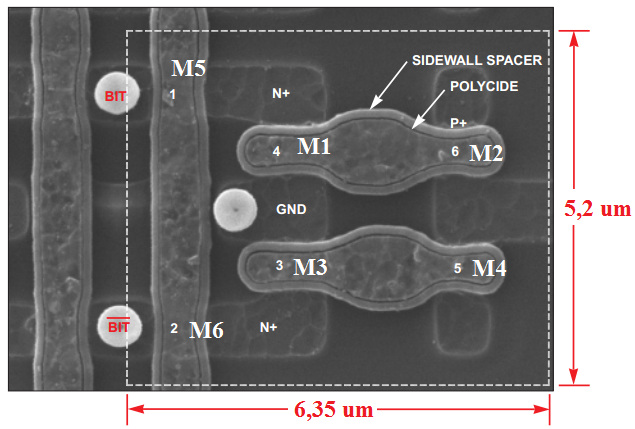
\includegraphics[width=0.4\linewidth]{common/memory/sram/sram-cell.jpg}
}

\begin{itemize}
\item Plně statické zapojení (kladná zpětná vazba)
\item Pro udržení informace vyžaduje napájení (volatilní paměť)
\item Nevýhoda, potřebuje 6 tranzistorů, velká plocha
\item Čtení, po výběru slova (world line -- WL) jsou data přenesena na příslušné nenapájené dráhy (bit line -- BL)
\item Při zápisu přes připojené bitové dráhy na log. 1 a log. 0 dojde k vnucení stavu vetším proudem než zajišťuje vnitřní smyčka
\end{itemize}

\end{frame}

\begin{frame}
\frametitle{Detail paměťové buňky dynamické paměti -- DRAM}

\hbox{
\includegraphics[width=0.4\linewidth]{generated/memory/dram/dram-cz.pdf}\hspace{0.1\linewidth}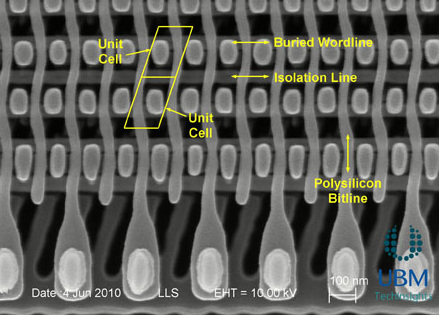
\includegraphics[width=0.4\linewidth]{common/memory/dram/dram-cell.jpg}
}

\begin{itemize}
\item nMOS tranzistor představuje přepínač, který připojí (nebo ne) kondenzátor na vodič „bitline“. Připojení je řízeno vodičem „wordline“.
\item Proces čtení kondenzátor vybíjí. Proto musí být poté obnoven.
\item Občerstvování pamětí (refresh) – náboj se z kondenzátoru samovolně ztrácí. Nezbytná pracovní fáze dynamické paměti. Negativně ovlivňuje (prodlužuje) průměrnou vybavovací dobu.
\end{itemize}

\end{frame}

\begin{frame}
\frametitle{Paměťová matice -- základ}

\centering

\includegraphics[width=1.0\linewidth]{generated/memory/sram/ram-matrix.pdf}

\end{frame}
